\chapter{GECO Concepts and Structure}

This section discusses 
\geco's approach to implementing GAs through a discussion of the classes, 
methods, and related functions it implements.

\section{Overview of \Geco\ Classes}

\Geco\ is an object-oriented library which implements an
environment primarily in the form of classes and methods. \Geco's classes are based
on the natural concepts which are part of the genetic evolutionary paradigm. The
principle classes form a hierarchy of {\em abstractions\index{\geco!abstraction
hierarchy}} ({\em not} a {\em class} hierarchy) which parallel the natural concepts
of genetic evolution. Objects which are higher in this abstraction hierarchy
`contain' objects which are lower in the hierarchy (see
Figure~\ref{fig:class-hierarchy}). We (GA developers) build on these classes and
methods to describe and implement our GAs. The terminology\index{\geco!terminology}
and concepts\index{\geco!concepts} used within \geco\ may differ slightly from other
conventional usage, but they hopefully are internally consistent, and should be
intuitive to a reader who is conversant with the concepts employed by GAs.

\begin{figure}[!htbp]
  \centering
  
\includegraphics[width=0.75\textwidth]{class-hierarchy.png}
  %
\includegraphics[]{class-hierarchy.png}
  \caption{\Geco's classes form an abstraction hierarchy}
  \label{fig:class-hierarchy}
\end{figure}

%% Note:
%% Using a .jpg image above without the width option causes the pagebreaking
%% algorithm to get busted by the big \samepage group below.
%% Using a .jpg above with the width option scales the image larger so much that
%% the pixelation of the image is objectionable. But the .pdf looks good!

Here are the principle classes in the \geco\ hierarchy of genetic 
abstractions, starting from the top:
{\samepage
\begin{description}
	\item [\inxclass{ecosystem}]\ hfill \break
	A combination of the population
	undergoing evolution, and the \term{genetic plan} which controls the evolution.

	\item [\inxclass{population}] \hfill \break
	GAs evolve populations of
	organisms.  The current population at any time is the set of organisms
	which can interact with one another to produce new organisms.
	
    \item [\inxclass{organism}] \hfill \break
    An organism combines all the related information
    about a single structure in the search space being explored by the
    GA. An organism is a member of a population, generally has a
    coded genetic description (its \concept{genotype}), and interacts with
    its environment as the individual (its \concept{phenotype}) coded by
    its genotype. Each organism also has a \concept{score}, which is used to
    establish an organism's relative value toward solving the specific
    problem posed for solution by the GA.

	\item [\inxclass{chromosome}] \hfill \break
	A structured component of an
	organism's genotype, which generally is the unit which is operated upon
	by \concept{genetic operator}s. Many GAs 
	use only a single chromosome per organism, but sometimes there are reasons to
	use more than one. Each chromosome is generally composed of a vector of
	\concept{loci} (sites), each of which may take on one of a set of values (the
	\concept{alleles} for that locus). The arity of each locus is typically the
	same for all loci of a single chromosome, but \geco is sufficiently general
	that arity may be a function of locus. Genetic interpretation is normally (but not
	necessarily) a function of position on the chromosome. 
   \begin{quote}
		Terminological aside:
		a \concept{gene} might be defined as a functional or operational unit by which
		genetic information is transferred from parent to offspring, which may
		consist of one or more alleles from one or more loci, which may or may not be
		contiguous on a chromosome. The exact definitions of genes and alleles in the context
		of GAs has historically been rather vague, but some attempts have been
		made to define them formally; see \cite{ga:radcliffe92-11,ga:radcliffe92-04}.
   \end{quote}
\end{description}
}%end \samepage

There are also some other important classes which, though they aren't part of the
gen\-et\-ic\-ly-based abstraction hierarchy, play important roles in \geco's operation.

\begin{description}

	\item[\inxclass{genetic-plan}] \hfill \break
	The overall strategy which determines how an
	ecosystem \term{regenerates}\index{regenerate}, \ie, how new organisms are created
	from older organisms. This generally includes the overall scheme for selection of
	organisms for reproduction, replacement, and manipulation by \term{genetic operator}s.
	Methods defined on this class will generally
	determine how a particular GA implementation differs from the canonical GA described
	by Holland. An instance of this class is a component of each ecosystem.
	
	\item [\inxclass{population-statistics}] \hfill \break
	Information accumulated about
	(at least) the \term{score}s of the members of a population, used for normalizing the scores
	across the population, \etc. An instance of this class is a component of each population.

\end{description}

{\samepage
In addition, there are other classes in \geco.  Some of these classes 
specialize on the classes above, while others serve auxiliary purposes.  

\begin{description}

\item [Organism Phenotype Mixin]
\ttdblinx{organism-phenotype-mixin}{Class}\index{phenotype} An \concept{abstract
class} (one not intended to be instantiated), which may be included as a parent
class in a subclass of the \inxclass{organism} class.\footnote{A \concept{mixin
class} is a class which is {\em mixed in} with other classes to collectively form
the set of parent classes of a new class. A mixin class is almost always an
\term{abstract class}.} This class adds a \inxslot{phenotype} slot to the subclass,
along with relevant behavior, when a phenotype must actually be generated from the
genotype. Since this is not always necessary, the \cl{phenotype} slot has been
abstracted out of the \cl{organism} class.

\item [Maximizing \& Minimizing Score Mixins] Two abstract classes, one of which
should be included as one of the superclasses of an application's population class.
That is, an instantiable subclass of \inxclass{population} must also be a subclass of
one of these classes (using multiple inheritance). The mixin you choose to include in
your population class will determine whether GECO tries to maximize or minimize the
organisms' scores in the population being evolved.

\item [Generational Population] A subclass of \inxclass{population} which provides
explicit support for the standard generational style of GA. Eventually \geco\ may
contains support for other styles of GA, possibly including parallel populations,
steady-state populations, \etc. This class (or a future alternative) should be included as
one of the superclasses of an application's population class.

\item [Binary Chromosome] A special kind of chromosome --- When each locus of a
chromosome may only take on one of two alleles, then each of the loci are binary, and the
chromosome which they compose is binary. It is very common for a GA to require only
binary chromosomes, and so \geco\ provides support for this special case.

\item [Sequence Chromosome] Another special kind of chromosome --- When each locus of the
chromosome is treated as a unique item of a sequence, and the chromosome itself specifies
a permutation of the sequence. This is another common kind of chromosome, used for
applications such as the Traveling Sales-rep Problem (TSP\index{TSP}).
	
\item [Gray Code Translation] \index{gray code} A special translation table for
converting to and from gray coded representations of a specific number of bits. Some
applications of GAs using binary chromosomes work better if the genetic coding scheme for
some parameters is a gray code.

\end{description}
}%end \samepage


\section{Basic Flow of Control}

Assuming that the appropriate definitions have been made to extend \geco\ 
for a specific GA implementation,  the basic operation of a typical GA is 
as follows:
{\samepage
\begin{description}
  \item[Initialization:] Make an instance of the ecosystem class or 
  subclass which will be used for the GA.  \Geco\ then automatically
  creates instances of the appropriate classes for the \term{genetic plan}
  and the \term{population}.  
  Creating the initial \inxclass{population} instance in turn causes the creation of 
  the initial \inxclass{organism} instances which belong to the population, each of 
  which is initialized with random chromosomes of the appropriate classes
  (see Figure~\ref{fig:initialization-tree}).
  \nopagebreak
  \item[Evolution:] Invoking \inxgeneric{evolve} on the ecosystem causes \geco\ to 
  evolve the population (see Figure~\ref{fig:evolve-tree}).
  This consists of repeating the following steps:
  \nopagebreak
  \begin{itemize}
    \nopagebreak
    \item \term{Evaluate}\index{evaluate} each of the organisms in the current population, recording 
    a \term{score} for each one.
    \item Calculate population statistics, normalized \term{score}s
    for each organism, and normalized population statistics.
    \nopagebreak
    \item Determine if the GAs termination condition has been met.  If 
    it has, then terminate.  Otherwise:
    \nopagebreak
    \begin{itemize}
      \nopagebreak
      \item \term{Regenerate}\index{regenerate} the population.  This is where most of the 
      customizing is done for a new GA in \geco.  This typically includes 
      selecting members of the previous population to participate in 
      creating the members of the new population.  \Geco\ provides a number 
      of predefined functions for performing the selection and for 
      creating the new population based on members of the previous one, 
      \eg, via reproduction, and various kinds of
      \concept{crossover} and \concept{mutate}.
      \nopagebreak
      \item Recursively\footnote{This recursive invocation could lead to 
                        `stack overflow' or similar error conditions in
                        many languages.  In Lisp, this particular kind
                        of recursion (called \concept{tail recursion})
                        is a special case which can be recognized by the
                        compiler and implemented (very efficiently) as
                        simple iteration. The result is an
						implementation which is concise, clear, and
						efficient. For those implementations which do not provide this
						optimization, an equivalent iterative definition is provided, which
						can be selected using conditional compilation
                        options specified in the \path|packages.lisp| file. See the
                        comments in that file for details, and also see Chapter~\ref{ch:geco-files}, page~\pageref{file:packages.lisp}}\label{recursive-vs-iterative-evolve}
      evolve the result. 
    \end{itemize}
  \end{itemize}
\end{description}
}%end \samepage

\begin{figure}
  \centering
  % 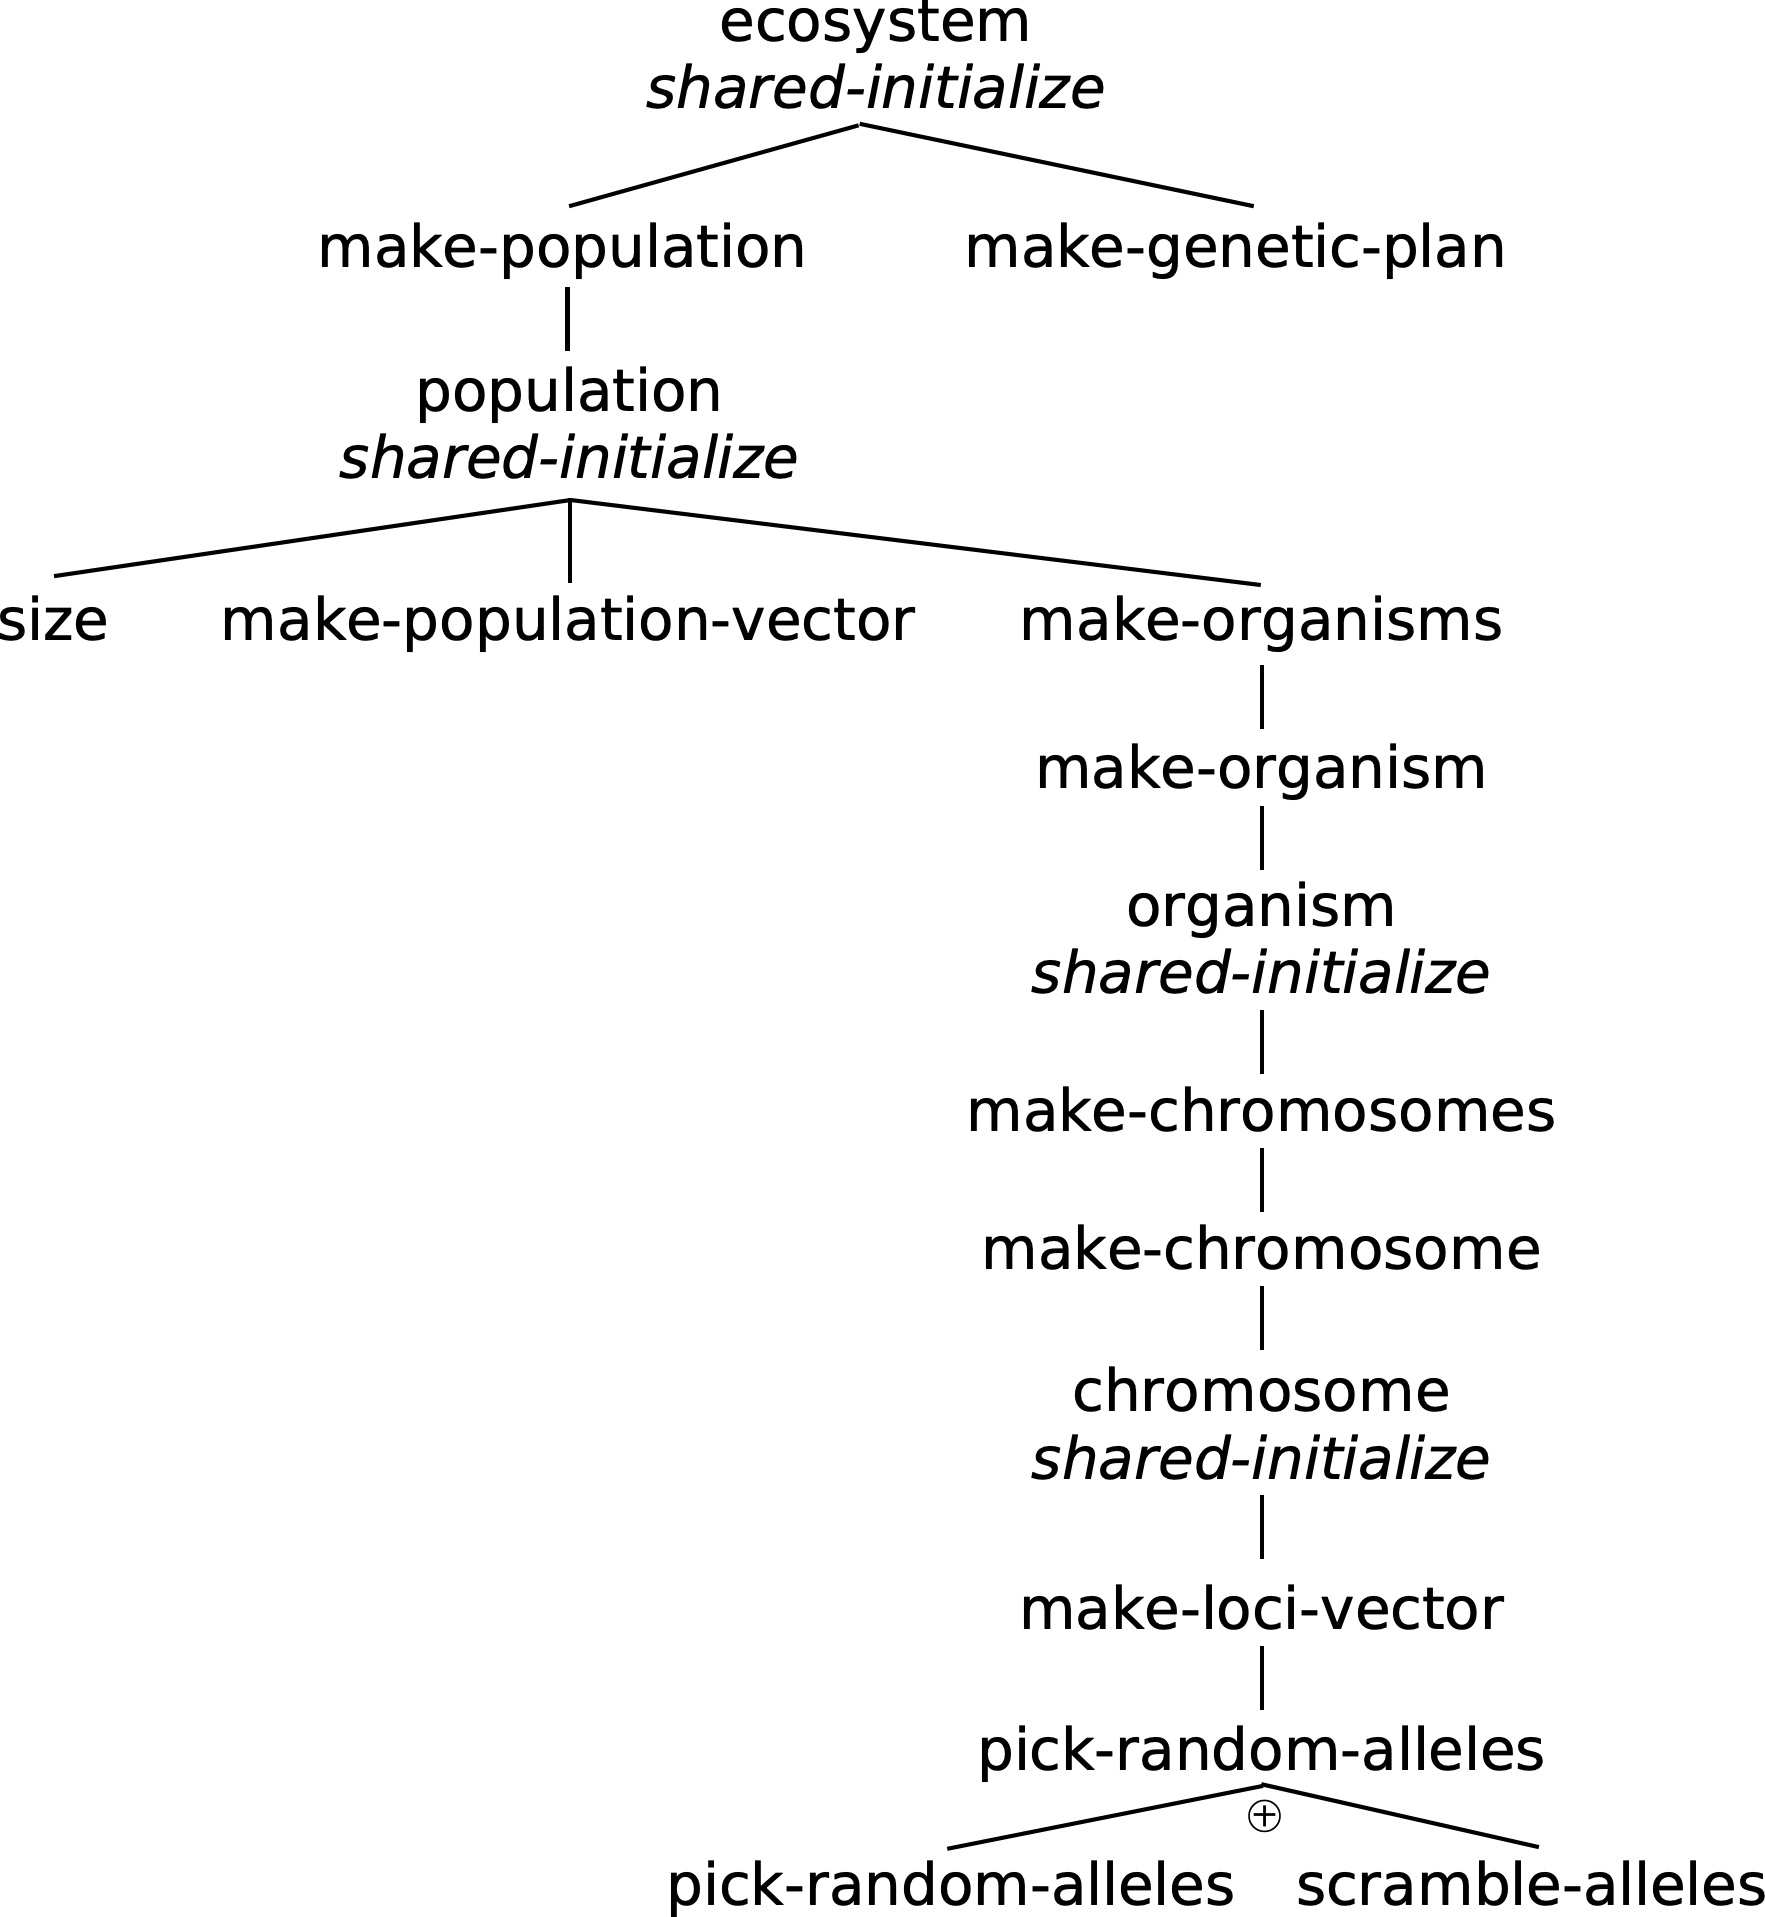
\includegraphics[width=\textwidth]{initialization-tree.eps}
  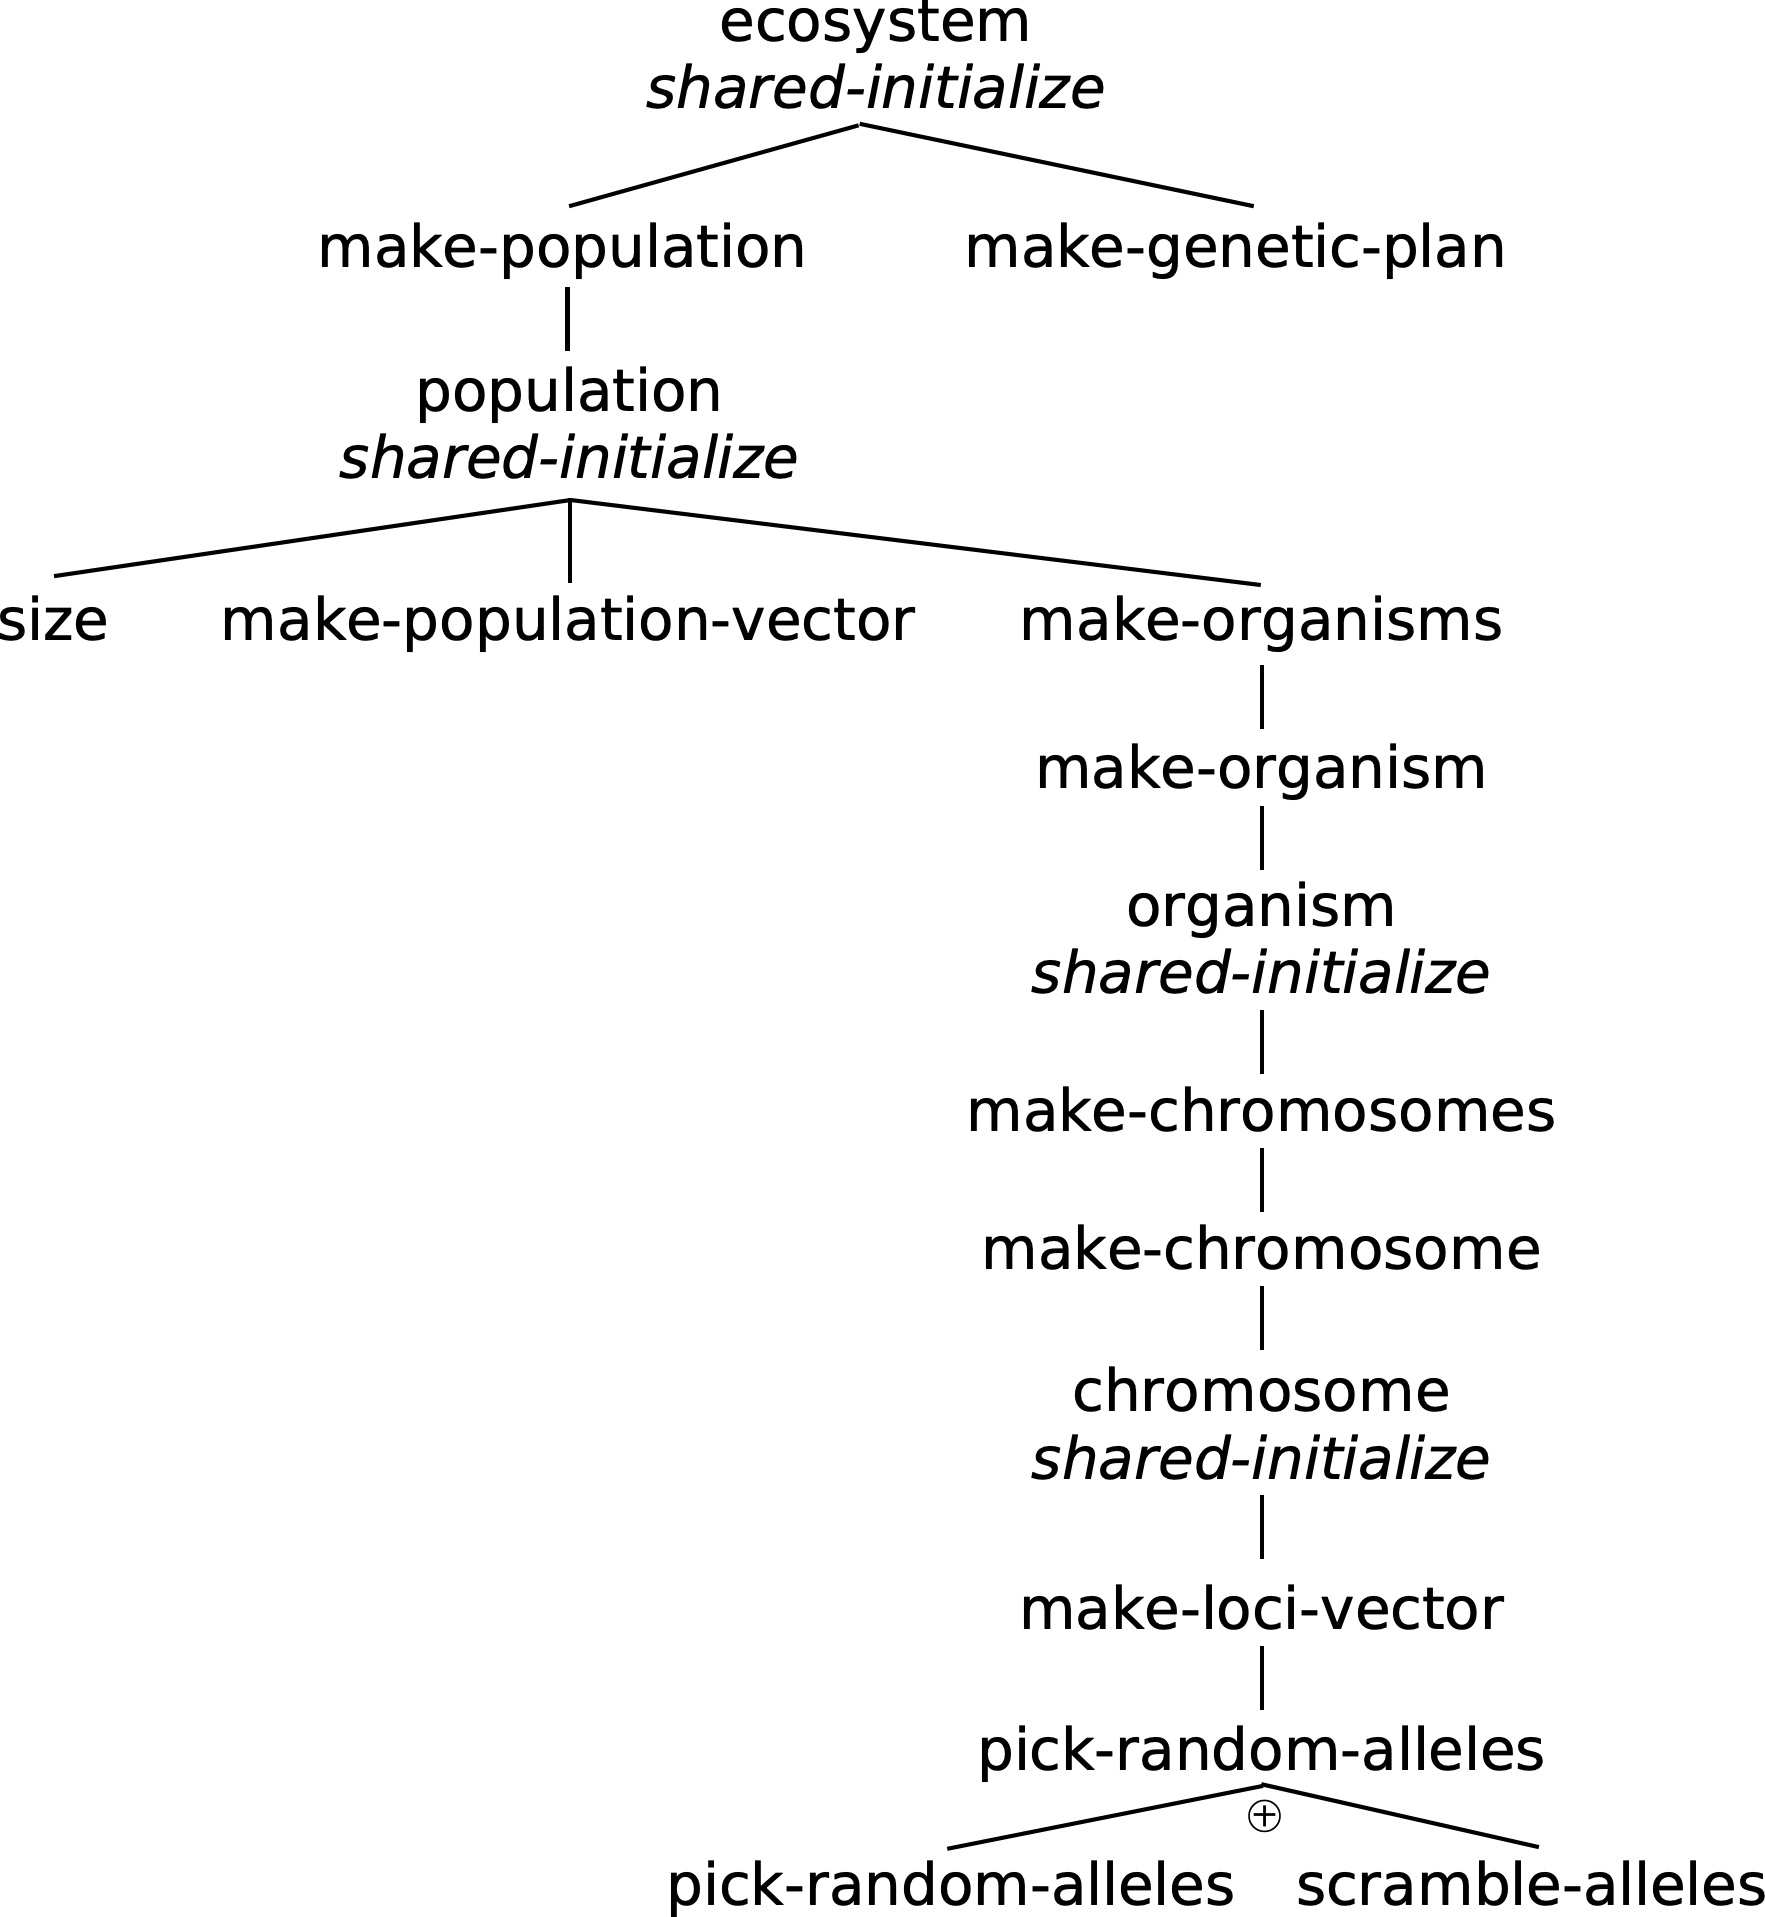
\includegraphics[width=0.6\textwidth]{initialization-tree.png}
  \caption{Call hierarchy for initialization of \Geco's principle structures}
  \label{fig:initialization-tree}
\end{figure}

\begin{figure}
  \centering
  % 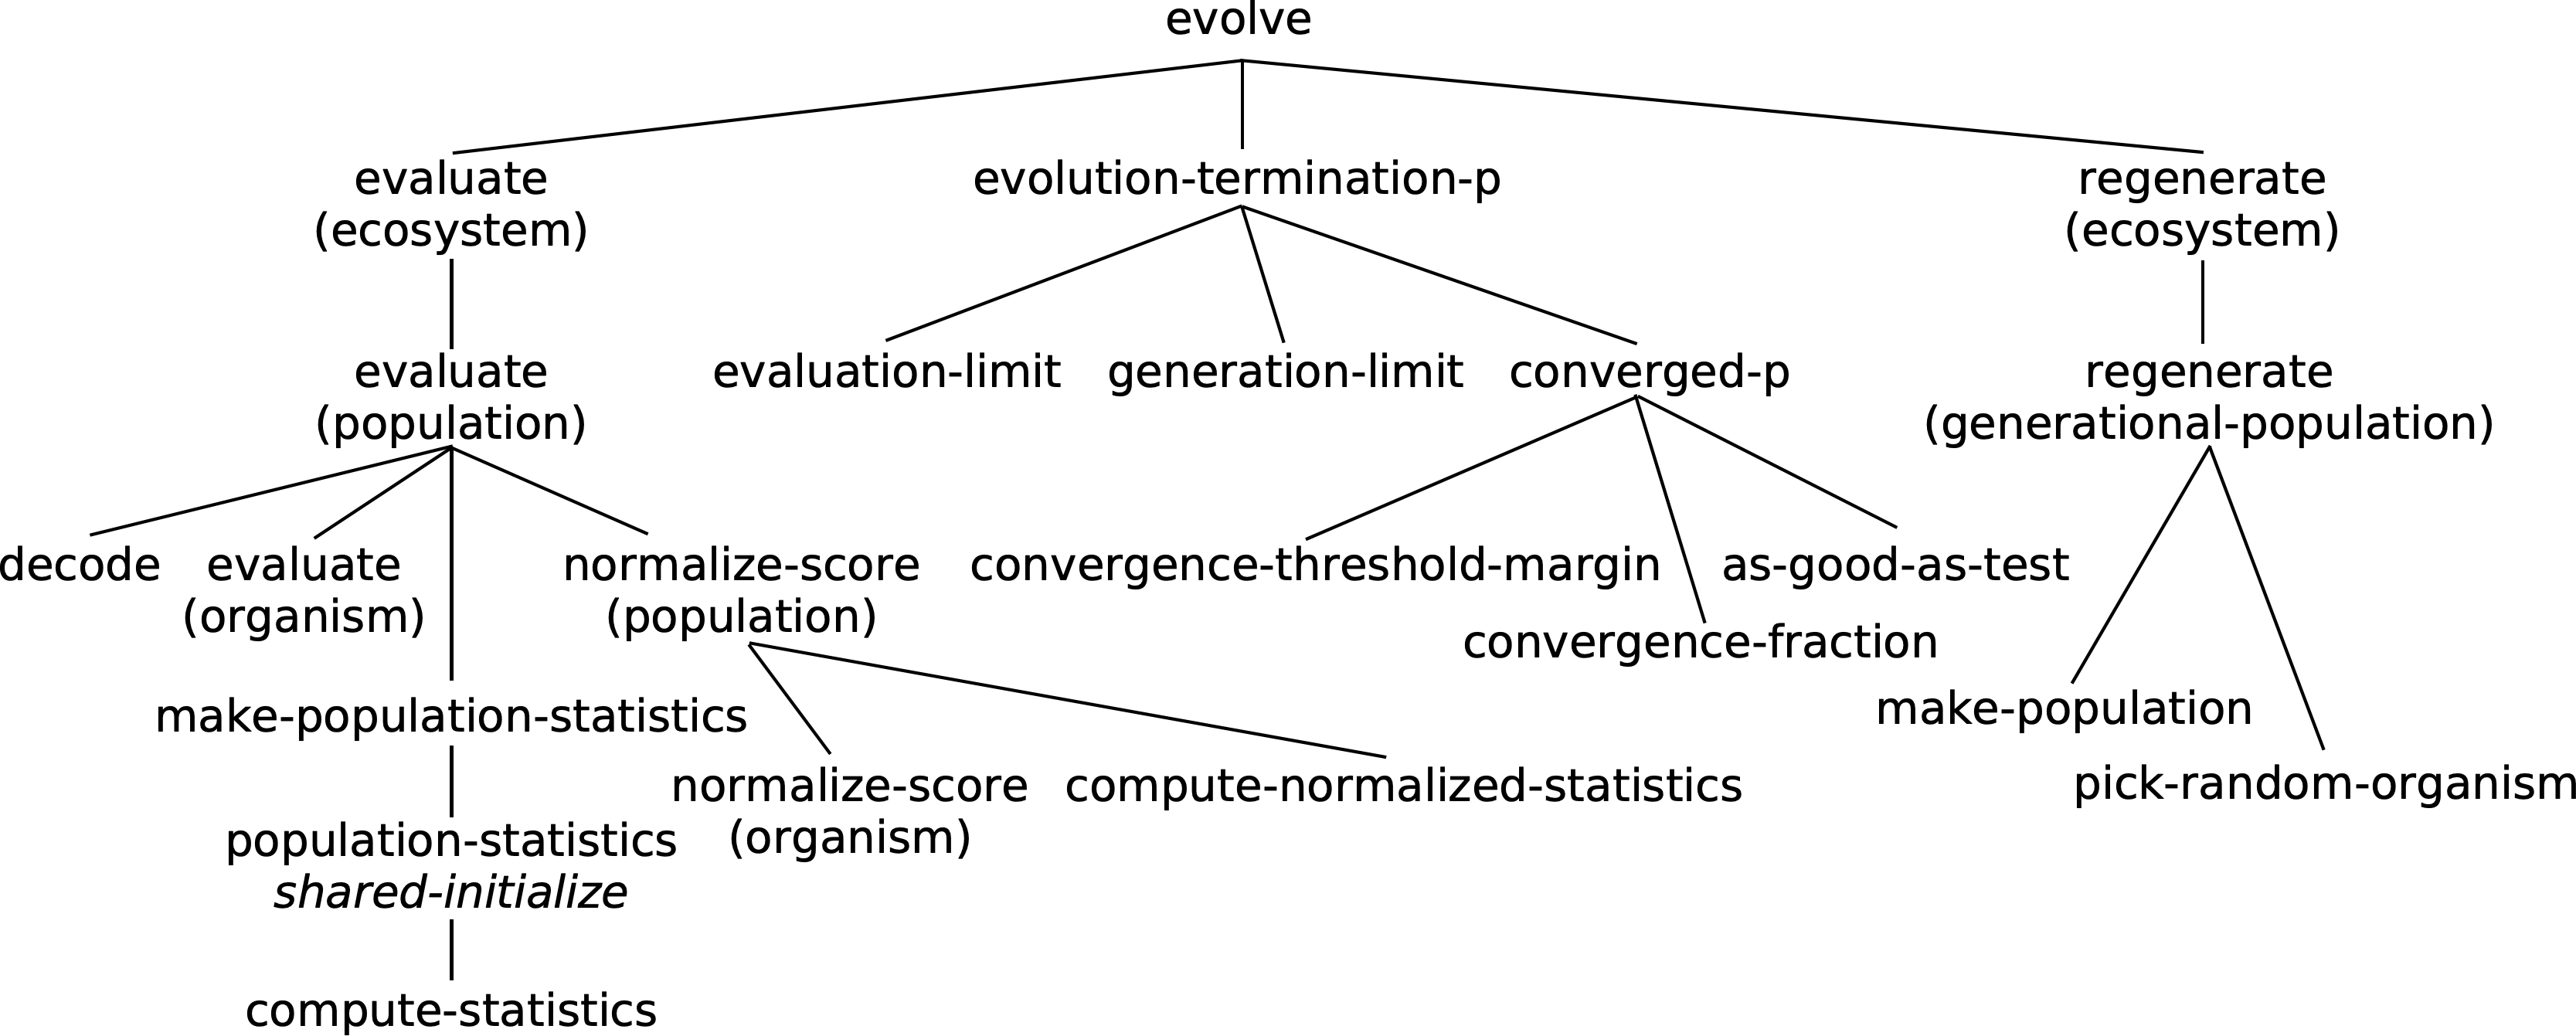
\includegraphics[width=\textwidth]{vert-evolve-tree.eps}
  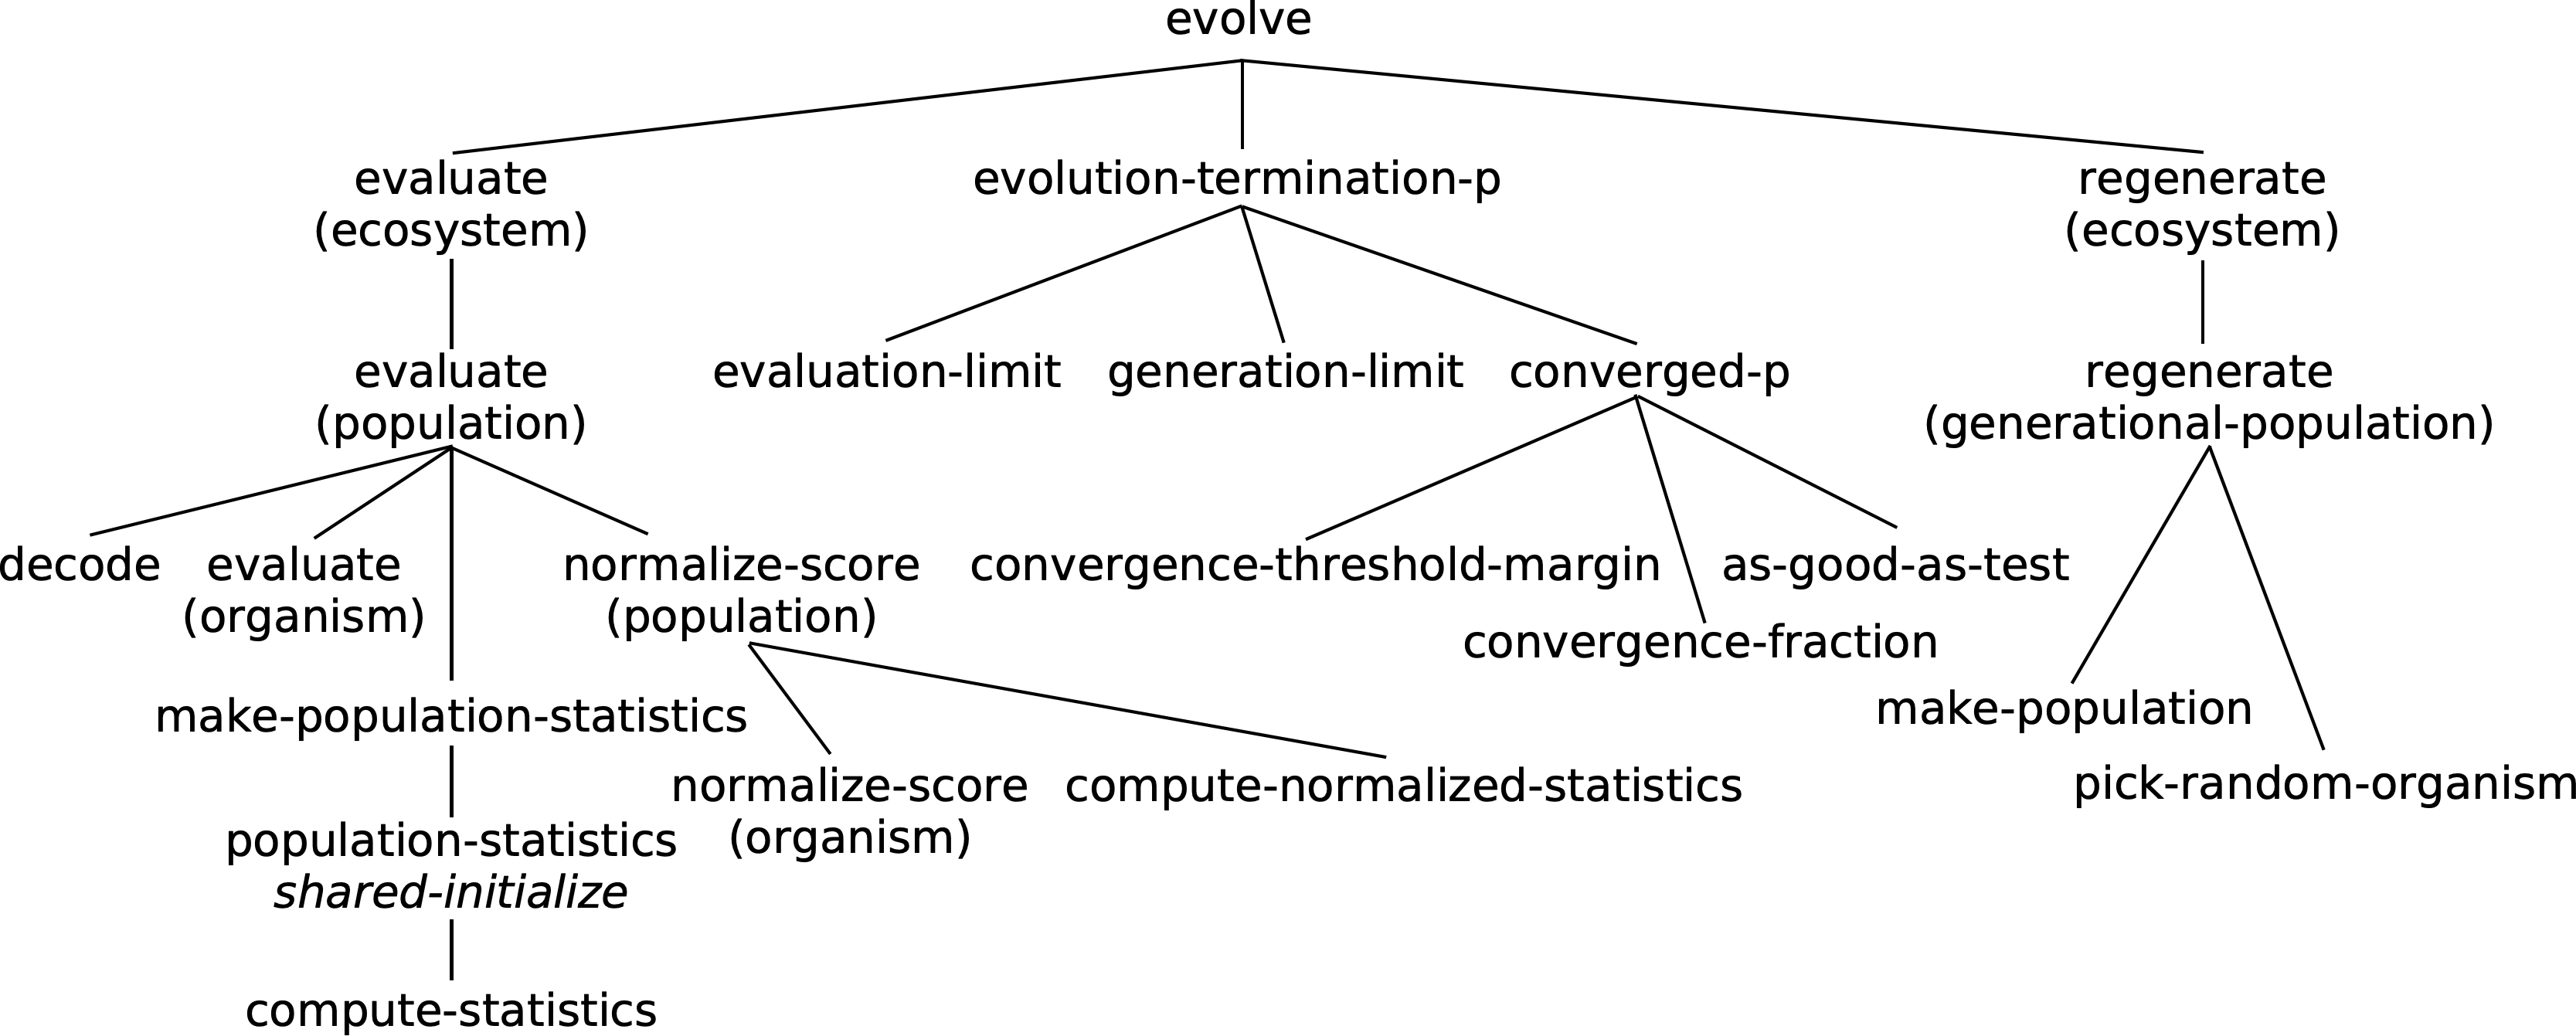
\includegraphics[width=\textwidth]{vert-evolve-tree.png}
  \caption{Call hierarchy for \Geco's evolutionary processing}
  \label{fig:evolve-tree}
\end{figure}

When supplied with the appropriate information, \geco\ can perform much of the
book-keeping, initialization, and control automatically.  This is made
possible by the built-in links between objects which are built upon the
\geco\ classes (see Figure~\ref{fig:class-interrelationships}).

\begin{figure}
  \centering	%% class-interrelationships.png is exported from class-interrelationships.pxd.pdf.cvd
  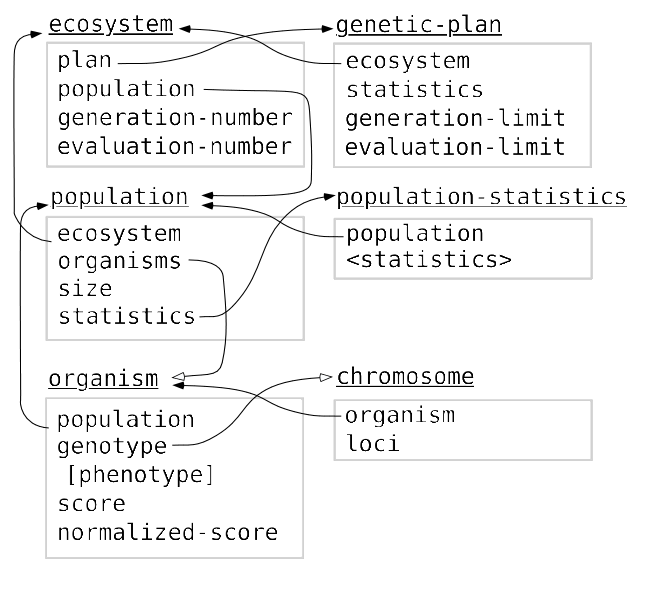
\includegraphics[width=0.75\textwidth]{class-interrelationships.png}
  % 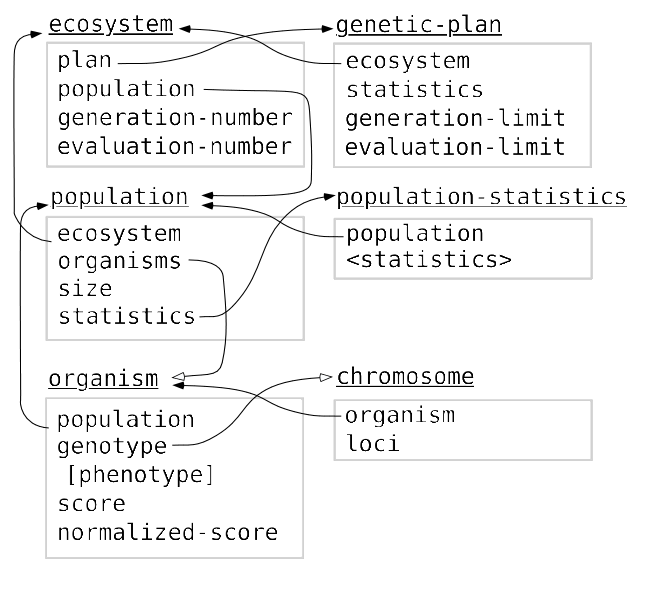
\includegraphics[]{class-interrelationships.png}
     \begin{center}
Solid head arrows indicate a one-to-one link;\\
hollow head arrows indicate a one-to-many link.
     \end{center}
  \caption{Interrelationships between \Geco\ objects}
  \label{fig:class-interrelationships}
\end{figure}


